\chapter{Einführung in Polymer}\label{einfuehrung-in-polymer}

Die Library Polymer setzt auf die in Kapitel \ref{web-components-nach-w3c} gezeigten Web-Components-Standards auf und soll den Umgang mit ihnen vereinfachen sowie deren Funktionalitäten erweitern. Dadurch will es Polymer ermöglichen, gekapselte Komponenten zu entwickeln, welche wiederum von Komponenten verwendet oder mit anderen Komponenten verbunden werden können. Diese Komponenten können dann zu einer komplexen Applikationen zusammengefügt werden. Der Name Polymer (``Poly'' - mehrere, ``mer'' - Teile) ist dabei eine Metapher für die Polymerisation von einzelnen Monomeren (den nativen \ac{HTML}-Elementen) zu einem großen Molekül (einer Web-Komponente). In diesem Kapitel wird in Abschnitt \ref{architektur} die Architektur der Library gezeigt, in Abschnitt \ref{elemente-katalog} wird der darauf aufsetzende Elemente-Katalog dargestellt.


\section{Architektur}\label{architektur}

Eine mit Hilfe von Polymer implementierte Komponente lässt sich in mehrere Schichten, wie in Abbildung \ref{fig:schimopo} dargestellt, unterteilen. Die Browser-Schicht stellt die nativen \ac{API}s der Web-Technologien dar, welche von der Polyfill-Schicht, den webcomponents.js-Polyfills (siehe Abschnitt \ref{polyfills-mit-webcomponents.js}), ersetzt oder erweitert werden können, falls der Browser die notwendige Technologie nicht unterstützt. Polymer kann dabei als Konformitäts-Schicht aufgefasst werden, welche auf die nativen Technologien bzw. den Polyfills aufsetzt und sich aus folgenden drei Schichten zusammensetzt \cite{citeulike:13915080}: Der \texttt{polymer-micro}-Schicht, welche die grundlegenden Funktionalitäten für das Erzeugen von Custom Elements bietet, der \texttt{polymer-mini}-Schicht, welche den Umgang mit einem lokalen \ac{DOM} in einer Polymer-Komponente erweitert und erleichtert, und zuletzt der \texttt{polymer-standard}-Schicht mit allgemeinen und zusätzlichen Funktionalitäten für den Umgang mit Web Components. Auf die Polymer-Schicht können die Polymer-Elemente aufgesetzt werden. Diese bilden eine weitere Schicht, welche durch den Elemente-Katalog \cite{citeulike:13916374} repräsentiert wird. In dem Elemente-Katalog sind diverse mit Polymer umgesetzte Komponenten - sowohl für das \ac{UI} als auch für Kernfunktionen zum Entwickeln von Applikationen - vorhanden.

\begin{figure}[h]
 \centering
 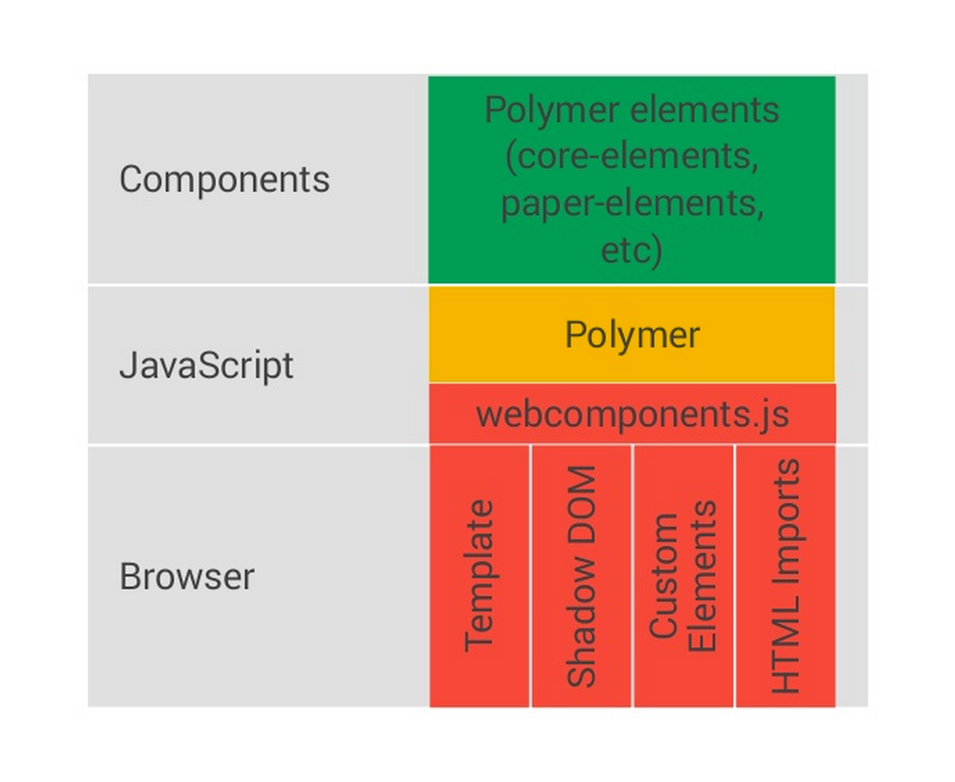
\includegraphics[width=7cm,keepaspectratio]{kapitel3/bilder/1-architektur}
 \caption{Schichtenmodell von Polymer}
 \label{fig:schimopo}
\end{figure}


\section{Elemente-Katalog}\label{elemente-katalog}

Der von Google verwaltete Elemente-Katalog verkörpert die Polymer-Philosophie ``There is an element for that'' \cite{citeulike:13930590}. Sie bilden eine Sammlung an Komponenten, welche die von Google vorgeschlagenen Implementierungen als Lösungen von einfachen bis komplexen wiederkehrenden Problemen sind. Entwickler können diese in ihrer eigenen Applikation optional einsetzen, sind aber beim Einsatz von Polymer nicht zwingend notwendig. Es werden dabei allerlei Anwendungsmöglichkeiten behandelt, von \ac{DOM}-Rendering in Form von Animationen, über Browser-\ac{API}-Interaktionen durch Push-Nachrichten, bis hin zu Remote-\ac{API}-Interaktionen mittels einem \ac{XHR}. Der Katalog besteht aus sieben Kategorien (Stand Januar 2016), welche die Komponenten nach Anwendungsfällen sortieren. Nachfolgend werden die Kategorien aufgelistet und erläutert.



\begin{description}
  \item[Iron Elements - Fe] Eisen ist der Kern der Erde. Daran orientiert sich die Metapher der Iron Elements, welche den Kern von Polymer und das Zentrum der Polymer Elemente bilden. Sie sind die wichtigsten Elemente, welche in vielen Projekten benötigt werden.
  \item[Paper Elements - Md] Die Paper Elements sind Googles-Design-Philosophie ``Material Design'' gehorchende Elemente wie Listen, Menüs und Tabs. Sie ermöglichen das Erstellen einer \ac{UI}. Paper ist dabei eine Metapher für ein erweitertes Papier, es kann zusammengesteckt werden, sich transformieren oder Schatten werfen.
  \item[Google Web Components - Go] Um die eigenen Services leichter verwendbar zu machen, stellt Google die Google Web Components bereit. Sie kapseln diese Services und \ac{API}s in Komponenten, wodurch Google Maps oder auch Google Drive usw. in der eigenen Applikation eingebunden und verwendet werden können.
  \item[Gold Elements - Au] Die Gold Elements sind eine Sammlung an buchstäblich wertvollen, goldenen Elementen, welche im Bereich E-Commerce eingesetzt werden können. Sie sind Komponenten für das Arbeiten mit Zahlungsmethoden oder Kreditkarteninformationen und können dabei Helfen, die Conversion-Rate der Applikation zu erhöhen.
  \item[Neon Elements - Ne] Die Neon Elements sind neben den Paper Elements auf \ac{UI}-Ebene einsetzbar. Mit ihnen können beispielsweise Animationen erstellt werden.
  \item[Platinum Elements - Pt] Wie die Gold Elements sind auch die Platinum Elements sehr wertvoll, jedoch in einer anderen Hinsicht. Sie sind nicht kommerziell orientiert, sondern für im Hintergrund laufende Services wie Push- oder Offline-Funk\-tio\-na\-li\-tä\-ten etc. gedacht. Sie sind Lösungen für sehr schwer lösbare, komplexe Probleme.
  \item[Molecules - Mo] Die Molecules sind weitere Elemente in Form von Wrappern für third-party-Lib\-rar\-ies.
  \item[Carbon Elements - C (in Entwicklung)] Die Carbon Elements befinden sich zum Stand dieser Arbeit noch in Entwicklung und sind noch nicht fertiggestellt. Sie sind metaphorisch sehr gewichtige Elemente und besitzen die Fähigkeit zur Bildung komplexer Moleküle, die essenziell für lebende Strukturen sind. Im übertragenen Sinn sind sie framework-orientierte Elemente und werden sich um strukturelle Probleme auf Applikations-Ebene kümmern.
\end{description}


\section{Alternative Sammlung von Komponenten}\label{alternative-sammlung-von-komponenten}

Statt den Polymer-Komponenten können auch selbst entwickelte oder aus anderen Quellen stammende Komponenten in eigenen Projekten verwendet werden. Der Elemente-Katalog wird dabei nur von Google vertrieben und erlaubt keine nicht von Google entwickelten Komponenten. Als eine Alternative für den Polymer Elemente-Katalog kann der customelements.io-Katalog \cite{citeulike:13926020} herangezogen werden. In diesem sind bereits mehrere tausend Komponenten gesammelt, welche von Google-unabhängigen Entwicklern für die unterschiedlichsten Anwendungsfälle entwickelt wurden.
